\documentclass{article}
\usepackage{float}
\usepackage{comment}
\usepackage{arxiv}
\usepackage[utf8]{inputenc} % allow utf-8 input
\usepackage[T1]{fontenc}    % use 8-bit T1 fonts
\usepackage{hyperref}       % hyperlinks
\usepackage{url}            % simple URL typesetting
\usepackage{booktabs}       % professional-quality tables
\usepackage{amsfonts}       % blackboard math symbols
\usepackage{nicefrac}       % compact symbols for 1/2, etc.
\usepackage{microtype}      % microtypography
\usepackage{lipsum}
\usepackage{graphicx}
\usepackage{braket}
\usepackage{array}      % Custom column widths
\usepackage{geometry}   % Adjust page margins
\usepackage{ragged2e}  
\usepackage{siunitx}

\usepackage[english]{babel}
\usepackage[square,numbers]{natbib}
\bibliographystyle{unsrt}
\usepackage{amssymb}
\NewDocumentCommand{\tens}{t_}
 {%
  \IfBooleanTF{#1}
   {\tensop}
   {\otimes}%
 }

\title{First principles studies of 7x7 graphene superlattices with topological defects and transition metal adatoms} %or 
%Quantum Machine Learning for Classification
% Enhancing Classification Algorithms with Quantum Machine Learning
% Classification via Quantum Machine Learning

\author{
 Sánchez Rolando \\
 School of Physical Sciences and Nanotechnology\\
 Yachay Tech University\\
 Urcuquí - Ecuador. \\
 \texttt{rolando.sanchez@yachaytech.edu.ec} \\
}


\begin{document}
\maketitle
\begin{abstract}
Graphene's unique properties have made it a promising material for many emerging areas. However, the absence of a bandgap and magnetic attributes restricts its potential for application in nanoelectronics and spintronics. These properties can be significantly altered by topological defects, such as Flower-Like Defects (FLD), which can also offer insights into their efficient applicability in those fields. Previous studies show that FLD in 5x5 and 6x6 supercells remove the characteristic Dirac cone, while in 7x7 supercells, the Dirac cone is recovered. Consequently, these findings prompt inquiries regarding the significance of defect size and symmetry in the electronic structure of graphene.
This study examines the impact of FLD in 7x7 supercells on the electronic properties of graphene and the additional modification of these properties by transition metal adatoms. Using density functional theory (DFT), we analyze changes in band structure, density of states, and magnetic properties. 
\end{abstract}

% keywords can be removed
\keywords{Graphene \and Flower-Like Defects \and Density Functional Theory \and Electronic Properties} 

\section{Introduction}
Graphene is one of the most fascinating materials known today. Its exceptional mechanical strength, thermal conductivity, and electron mobility make it a prime candidate for next-generation technologies. However, its lack of a bandgap and non-magnetic character significantly limit its application in areas like nanoelectronics and spintronics.

Previous studies carried out by our group investigated the effects of FLDs embedded in periodic graphene supercells. In these studies, it was observed that:
\begin{itemize}
    \item In $5\times 5$ and $6 \times 6$ supercells, FLDs disrupted the Dirac cone.
    \item But in $7\times7$ supercells, the Dirac cone re-emerged.
\end{itemize}

Now, graphene's lack of a bandgap and magnetism limits its applications in several fields, including electronics and spintronics. Topological defects, such as flower-like defects (FLDs) observed via scanning tunneling microscopy (STM) \cite{cockayne2011}, can modify these properties. One-dimensional extended defects also exhibit unique behaviors like one-dimensional conductivity \cite{pinto2014}. A systematic study of graphene's structural, mechanical, electronic, and magnetic properties is crucial to overcoming these limitations. In this study, we investigate a hexagonal array of FLDs forming a $7\times7$ superlattice to understand their influence on graphene's electronic properties.


\section{Methodology}
The calculations were performed using the Vienna Ab-initio Simulation Package (VASP) \cite{kresse1996}, employing the \textit{R2SCAN+rvv10} functional \cite{furness2020}. Visualizations were generated using VESTA \cite{momma2011} as shown in Figure \ref{fig:pristine}. We used a $900 \, eV$ plane-wave cutoff and a k-point mesh spacing of $0.022 \, \si{\angstrom}^{-1}$ for both pristine graphene and the $7\times7$ FLD superlattice.


\begin{figure}[H]
  \centering
  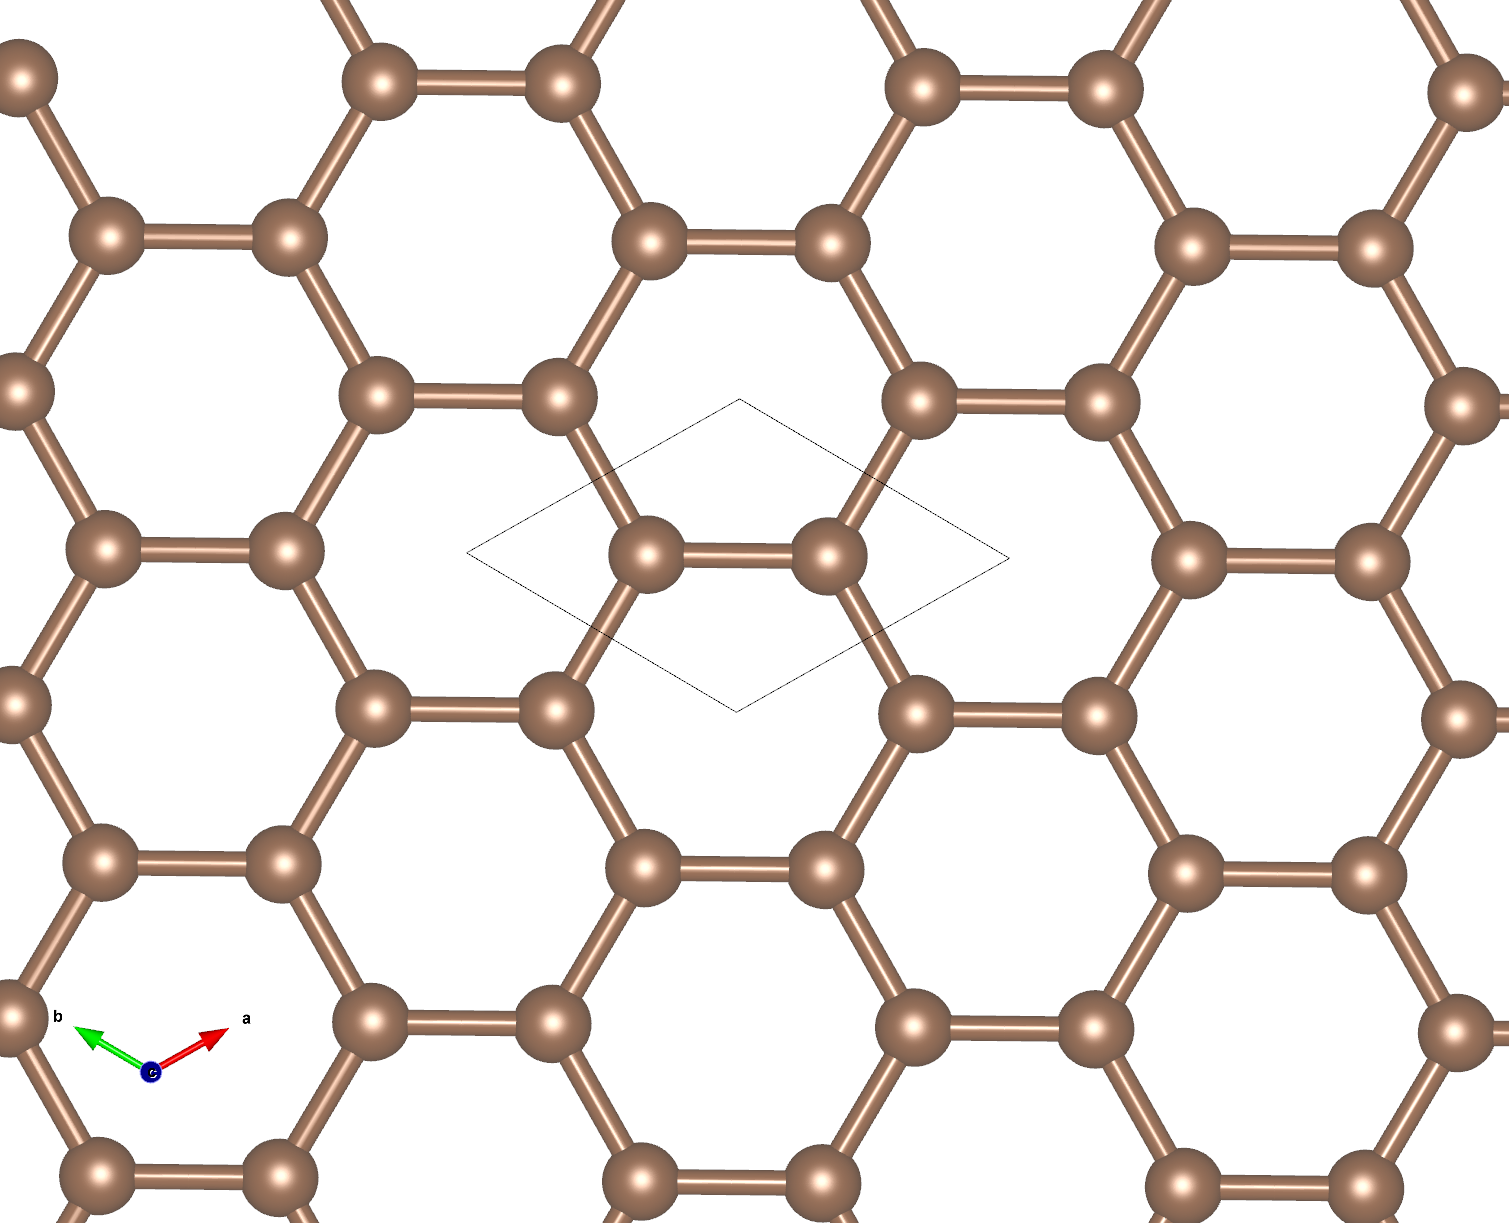
\includegraphics[scale=0.15]{../figures/pristine_structure.png}
  \caption{Graphical representation of pristine lattice.}
  \label{fig:pristine}
\end{figure}

\subsection{Convergence Criteria}
To ensure the accuracy of our calculations, we established convergence criteria of less than $1 \, meV$ for the total energy per atom. This criterion was applied to the k-point mesh and the energy cutoff (ENCUT) as shown in Figure \ref{fig:convergence}.

\begin{figure}[H]
    \centering
    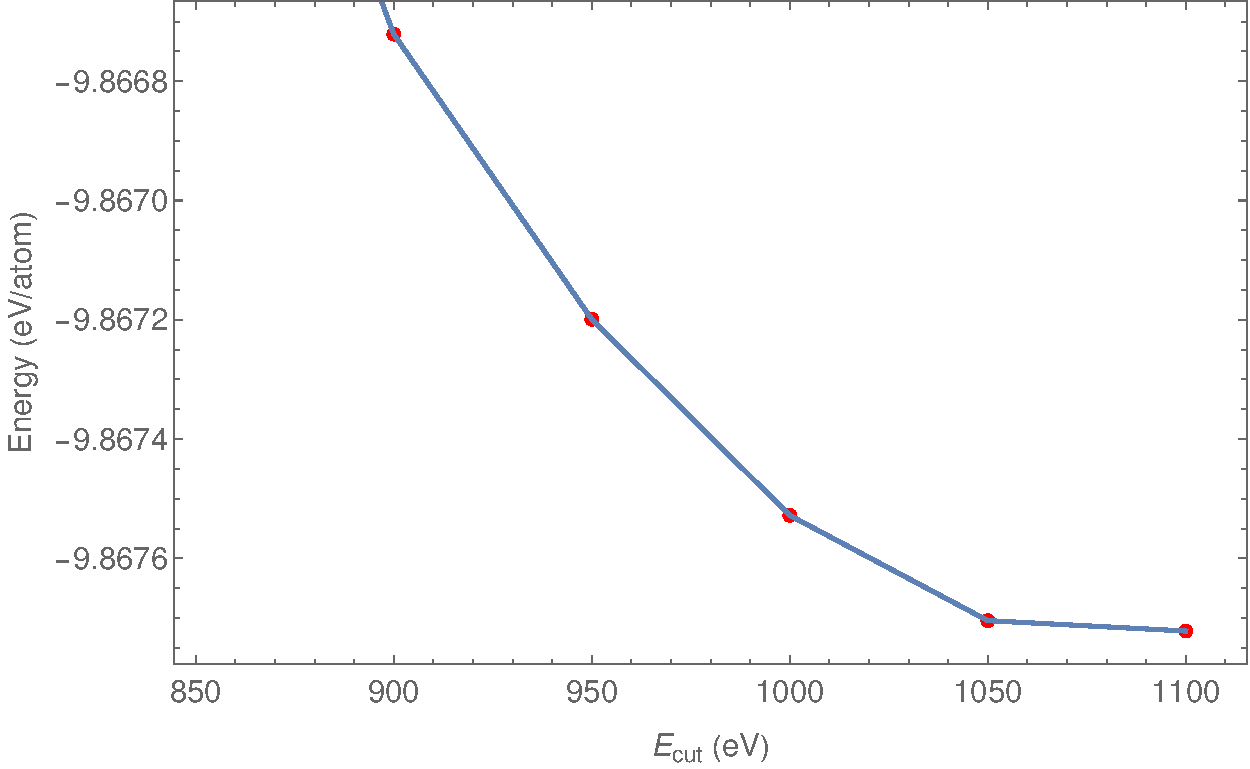
\includegraphics[scale=0.35]{../figures/p_encut.pdf}
    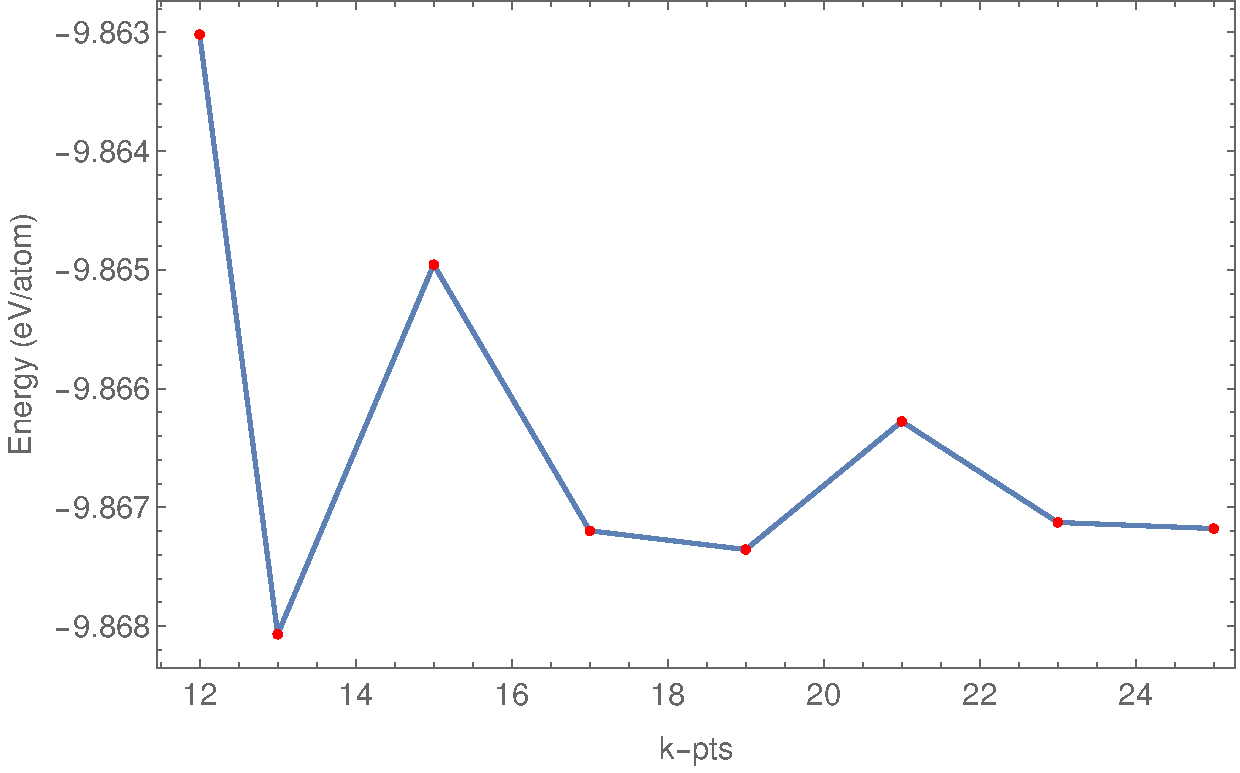
\includegraphics[scale=0.35]{../figures/p_kp.pdf}
    \caption{Convergence window of the total energy per atom with respect to the energy cutoff and number of k-points.}
    \label{fig:convergence}
\end{figure}

\section{Results}
\subsection{Pristine Graphene}
We began our analysis by examining pristine graphene, which serves as a reference for our study. The energy equation of state (EOS) for pristine graphene was obtained from Andrew, et al. \cite{Andrew2012}, then our calculated data was fitted to it as shown in Figure \ref{fig:pristine_eos}. From here, we infered mechanical properties such as the layer modulus, the force per unit length derivative, and the second derivative of the layer modulus as shown in Table \ref{table:eos}.

\begin{figure}[H]
  \centering
  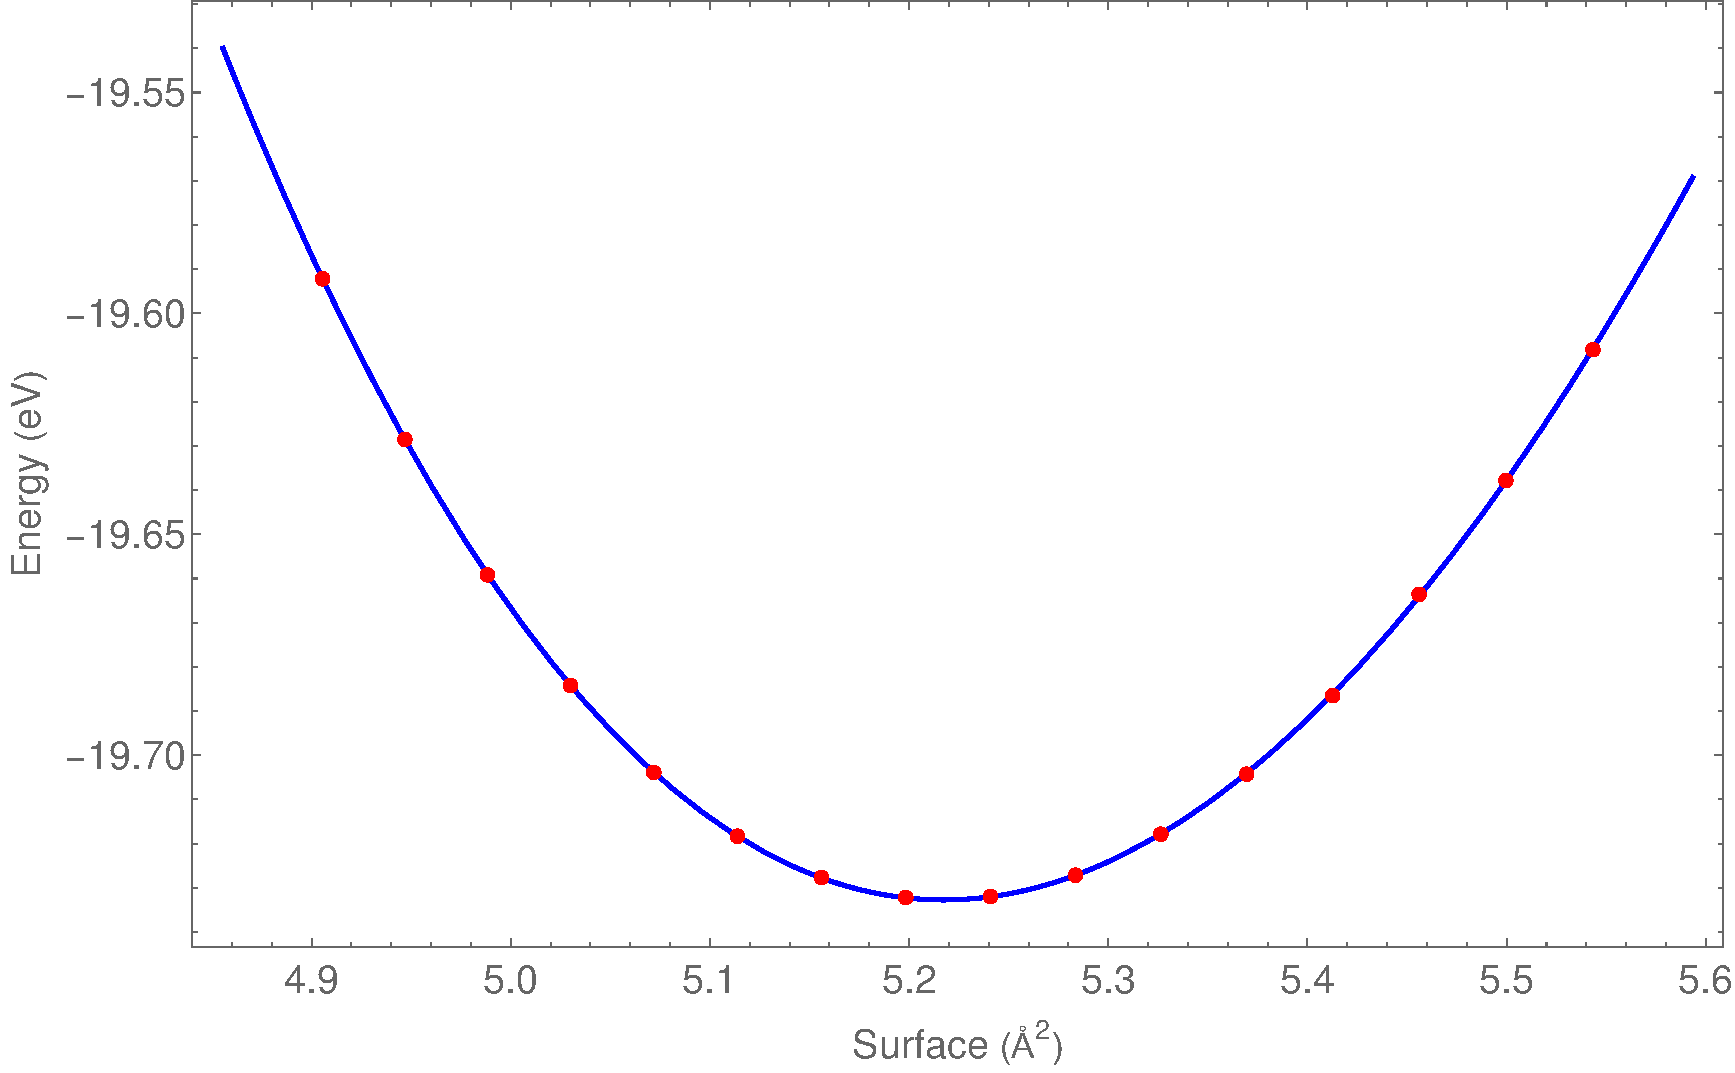
\includegraphics[scale=0.3]{../figures/p_eos.pdf}  
  \caption{Fitted energy EOS for pristine graphene.}
  \label{fig:pristine_eos}
\end{figure}

\begin{table}[]
  \centering
  \caption{Mechanical properties of pristine graphene.}
  \begin{tabular}{@{}ccccccc@{}}
  \toprule
  \textbf{System} & $a_{opt}$ & $N_{atom}$ & $\gamma \, (eV/\si{\angstrom}^2)$ & $\gamma'$ & $\gamma'' (\si{\angstrom}^2/ eV)$ & $E_{gap}$  \\ \midrule
  Pristine        & 2.454            & 2              & 13.51                  & 4.47             & -0.34  & 0              \\
  \end{tabular}
  \label{table:eos}
\end{table}

Then, we ran calculations on the band structure, density of states for pristine graphene, and create STM simulated images, as presented in Figure \ref{fig:pristine_e}. We can obseve the characteristic Dirac cone at the Fermi level and, in the partial density of states (PDOS) shown in Figure \ref{fig:p_pdos}, the $p_z$ being the only orbital contributting to near the Fermi level. These results are consisten with previous knowledge of pristine's electronic properties. 
\begin{figure}[H]
  \centering
  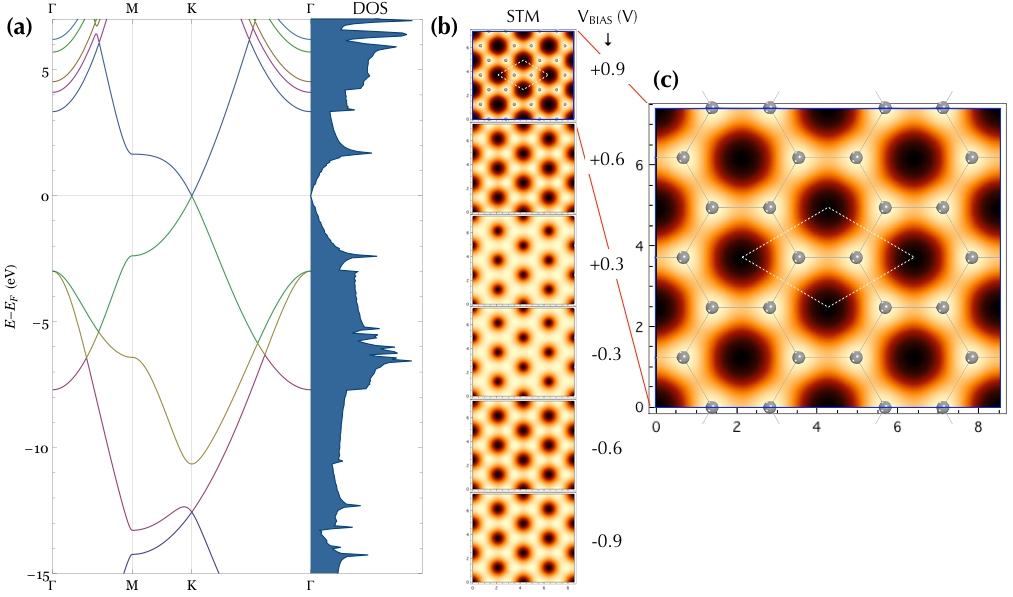
\includegraphics[scale=0.45]{../figures/pristine_bs_dos.jpg}  
  \caption{(a) Band Structure and Density of States (DOS) for pristine. (b, c) Simulated STM images for each corresponding VBIAS.}
  \label{fig:pristine_e}
\end{figure}
\begin{figure}[H]
  \centering
  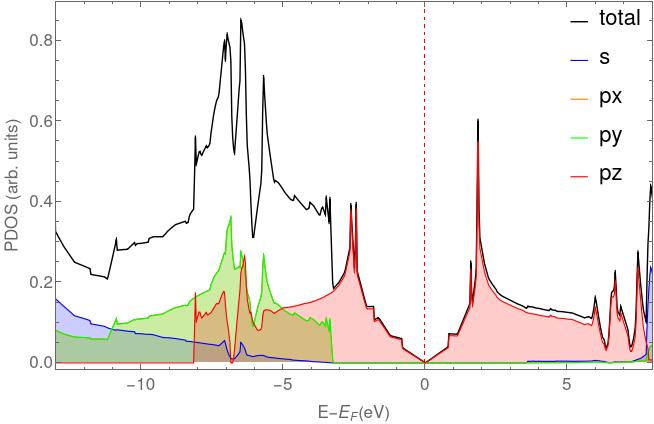
\includegraphics[scale=0.4]{../figures/pdos_pristine.jpeg}
  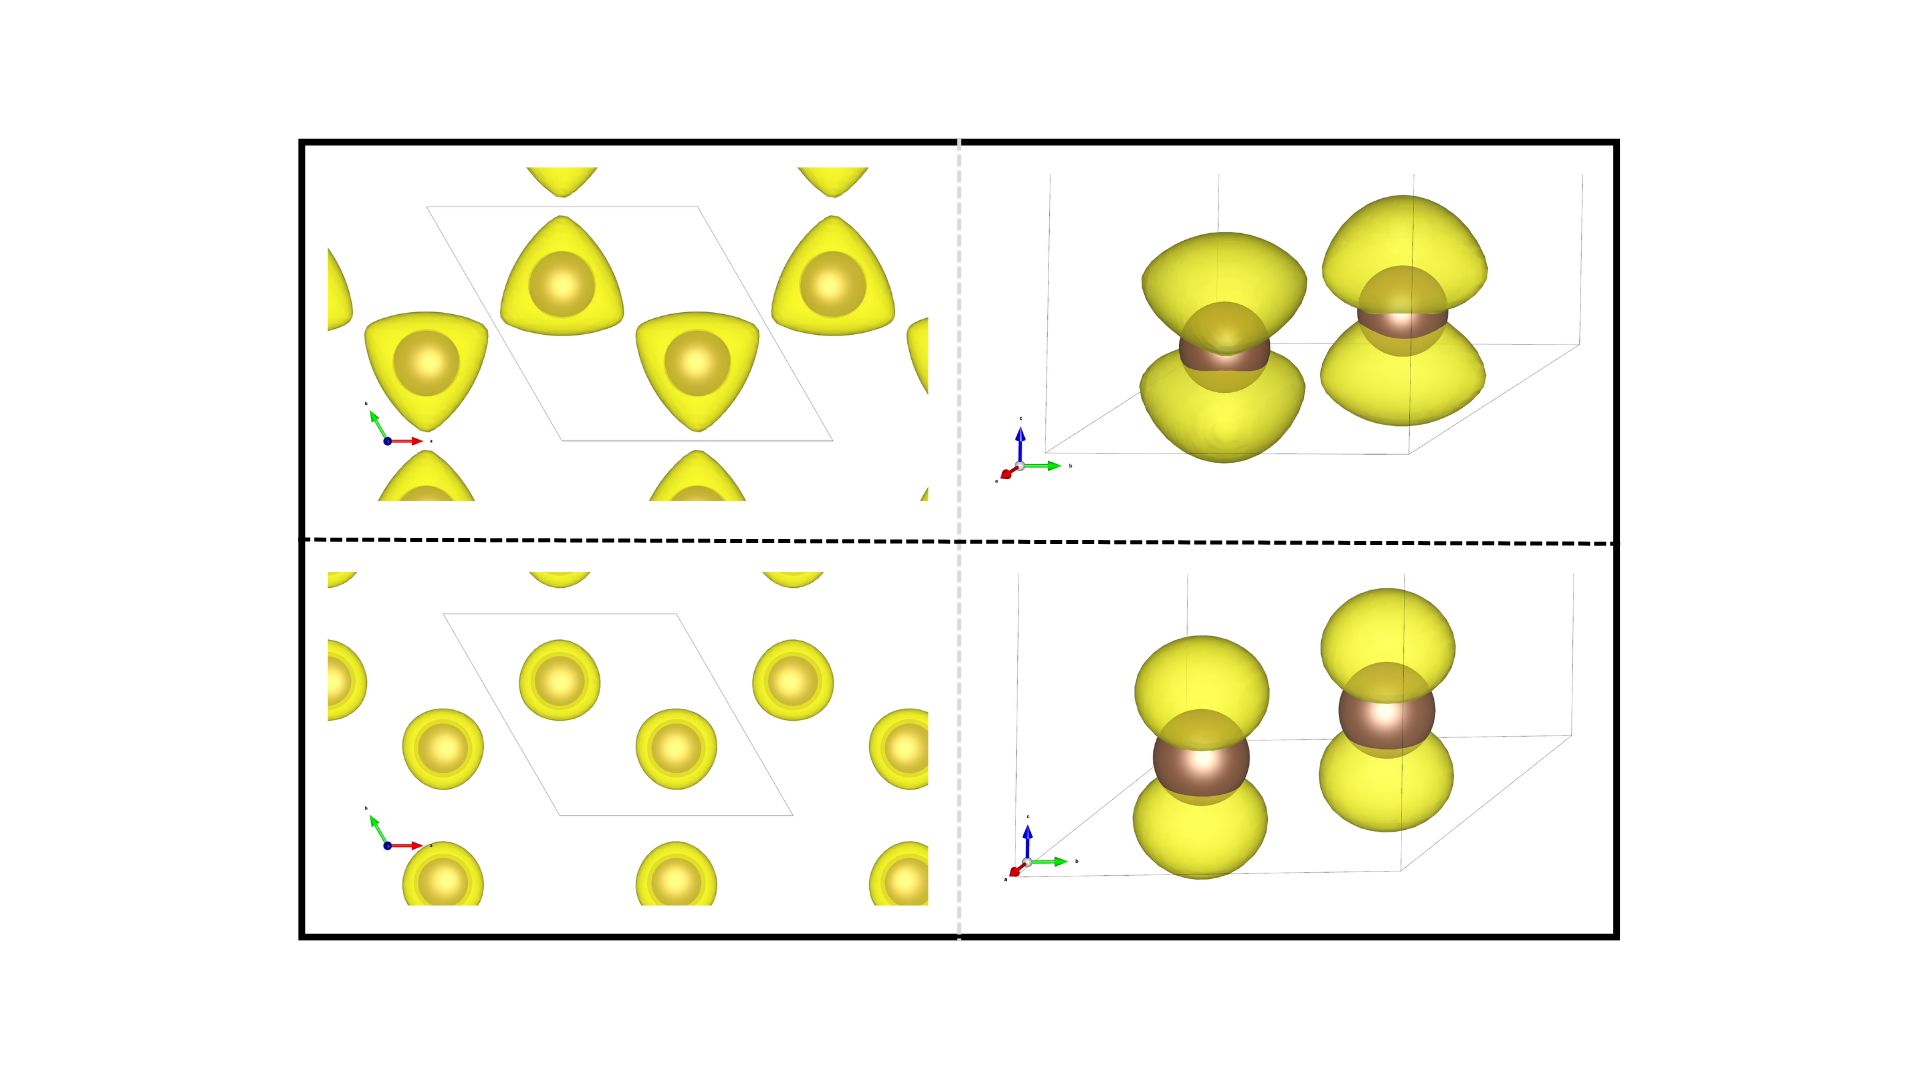
\includegraphics[scale=0.18]{../figures/parchg_pristine.png}
  \caption{Left: PDOS for pristine graphene. Right: (Top) Isosurface images of partial charge
  density of last occupied band. (Bottom) Isosurface images of partial charge density of first unoccupied band.}
  \label{fig:p_pdos}
\end{figure}

\subsection{\texorpdfstring{$7\times7$}{7x7} FLD Superlattice}
Figure \ref{fig:system} presents the $7 \times 7$ FLD superlattice structure. The corresponding energy--volume equation of state (EOS) fit is shown in Figure~\ref{fig:7x7_eos}, and the derived mechanical properties are summarized in Table~\ref{table:7_eos}. The electronic band structure and partial density of states (PDOS) are depicted in Figure~\ref{fig:7x7_band}, while simulated scanning tunneling microscopy (STM) images under various bias voltages are presented in Figure~\ref{fig:stm}.

From the calculated band structure and PDOS, the characteristic Dirac cone is clearly preserved, indicating that the semimetallic nature of graphene is maintained in the $7 \times 7$ FLD superlattice. The PDOS further shows that the states near the Fermi level are primarily derived from the $p_z$ orbitals of the carbon atoms within the FLD regions, highlighting their dominant role in shaping the low-energy electronic structure.

To further investigate the spatial distribution of these electronic states, we computed the isosurface images of the partial charge density associated with the valence band maximum (VBM) and conduction band minimum (CBM), shown in Figure \ref{fig:7iso}. The isosurface corresponding to the VBM reveals a noticeable localization of electronic density around the outer regions of the FLD, suggesting that the defect geometry modulates the spatial character of the occupied states. Finally, Figure~\ref{fig:stm} presents the computed STM image for the $7 \times 7$ defect array under a bias voltage of $V_{\text{bias}} = -0.3~\text{eV}$, offering a simulated topographic contrast consistent with the presence and periodicity of the FLD structures.

\begin{figure}[H]
  \centering
  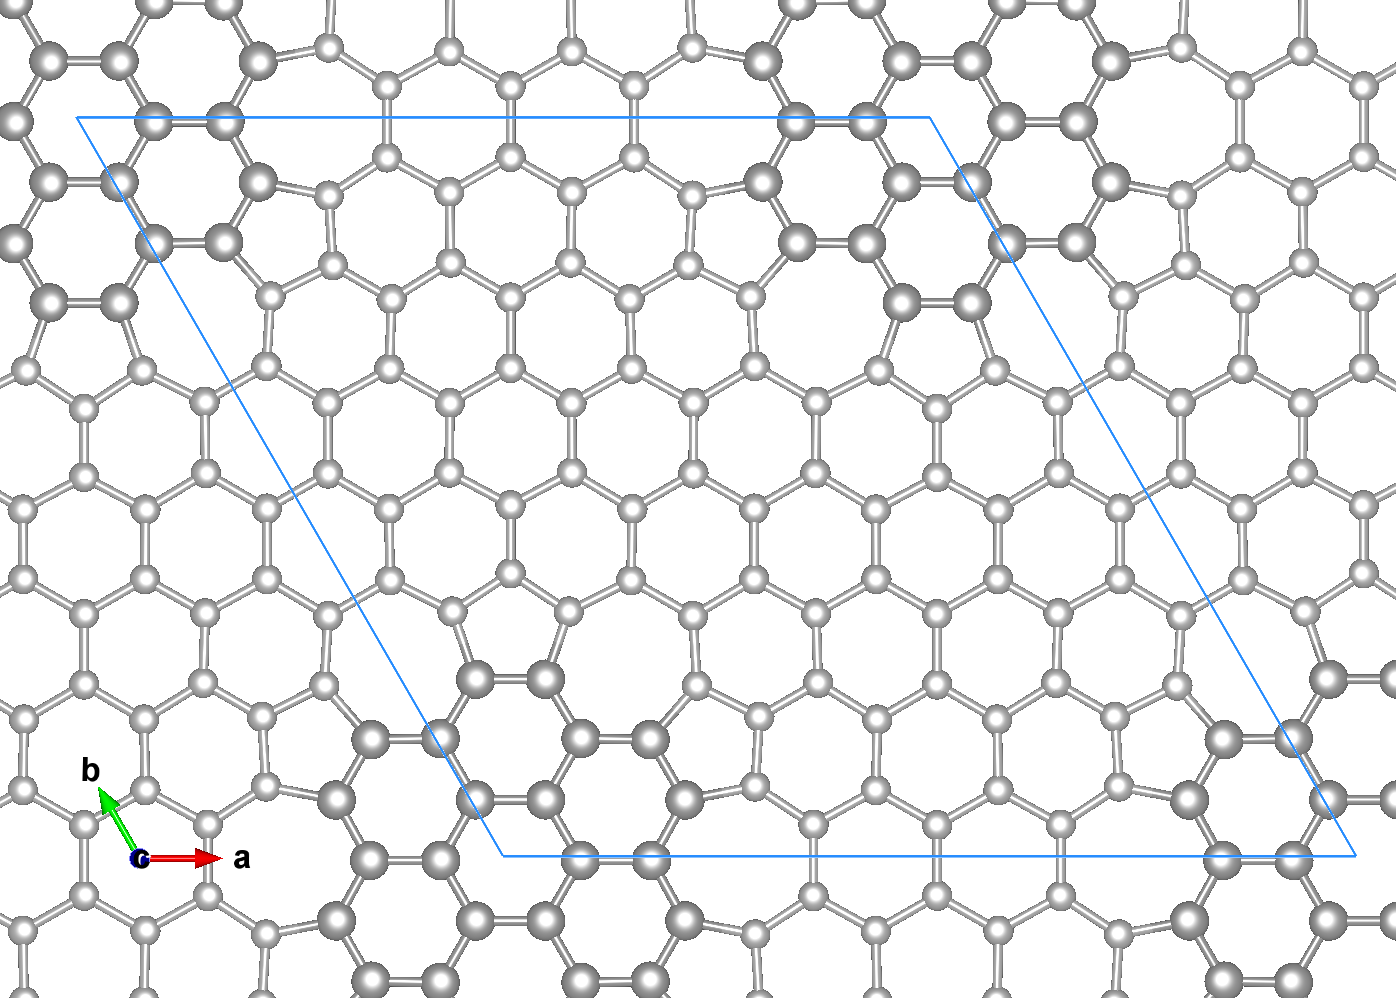
\includegraphics[scale=0.2]{../figures/7x7_FLD.png}
  \caption{Graphical representation of the 7x7 superlattice with FLDs. The highlithed spheres represent the FLD's carbon atoms.}
  \label{fig:system}
\end{figure}

\begin{table}[H]
  \centering
  \caption{Mechanical properties of $7\times7$ FLD superlattice.}
  \begin{tabular}{@{}ccccccc@{}}
  \toprule
  \textbf{System} & $a_{opt}$ & $N_{atom}$ & $\gamma \, (eV/\si{\angstrom}^2)$ & $\gamma'$ & $\gamma'' (\si{\angstrom}^2/ eV)$ & $E_{gap}$  \\ \midrule
  $7\times7$        & 17.262           & 98              & 13.24                  & 4.4.36             & -0.35  & 0              \\
  \end{tabular}
  \label{table:7_eos}
\end{table}
\begin{figure}[H]
  \centering
  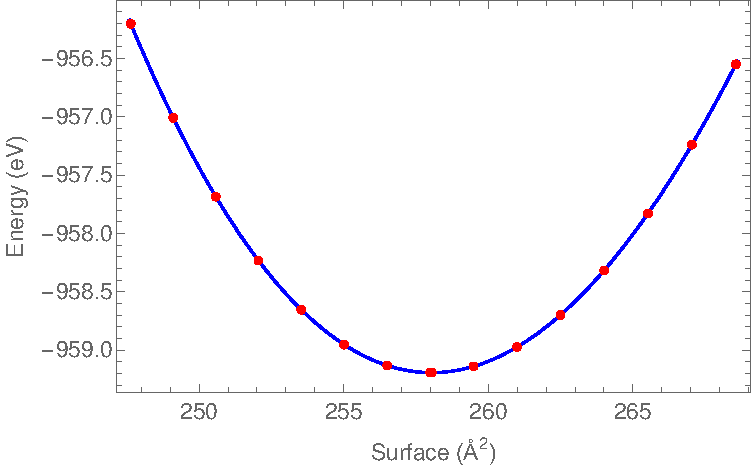
\includegraphics[scale=0.5]{../figures/7_eos.pdf}  
  \caption{Fitted energy EOS for superlattice.}
  \label{fig:7x7_eos}
\end{figure}
\begin{figure}[H]
  \centering
  \begin{minipage}{0.48\textwidth}
    \centering
    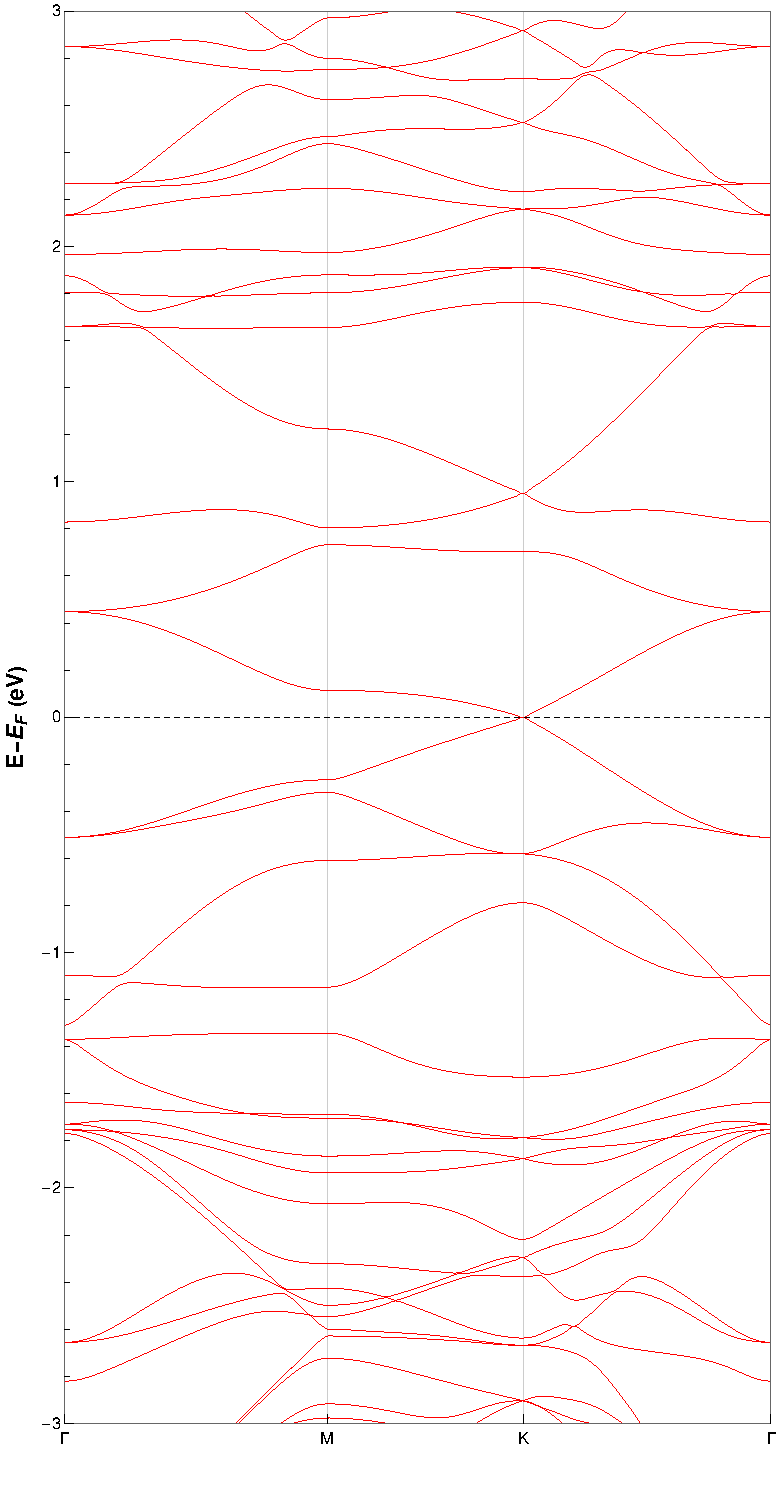
\includegraphics[scale=0.4]{../figures/7bs.pdf}
  \end{minipage}
  \begin{minipage}{0.48\textwidth}
    \centering
    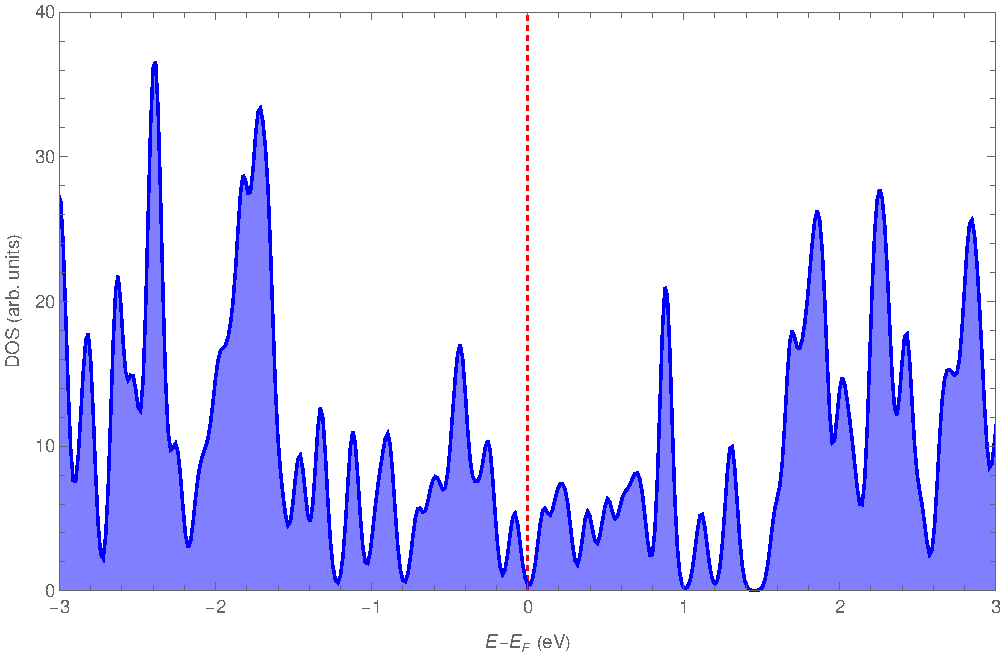
\includegraphics[scale=0.3]{../figures/dos7.pdf} \\[0.5em]
    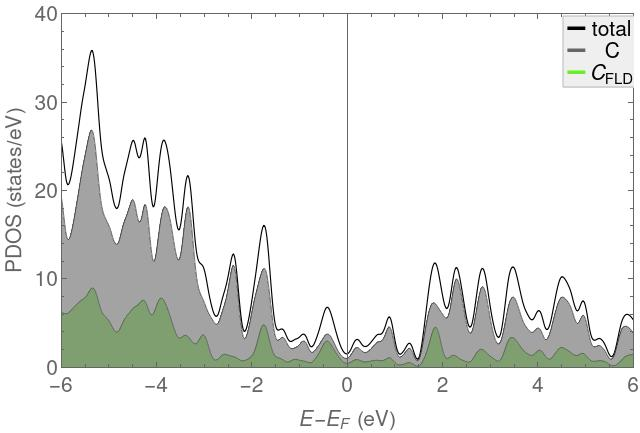
\includegraphics[scale=0.3]{../figures/pdos_7x7.jpeg} \\[0.5em]
    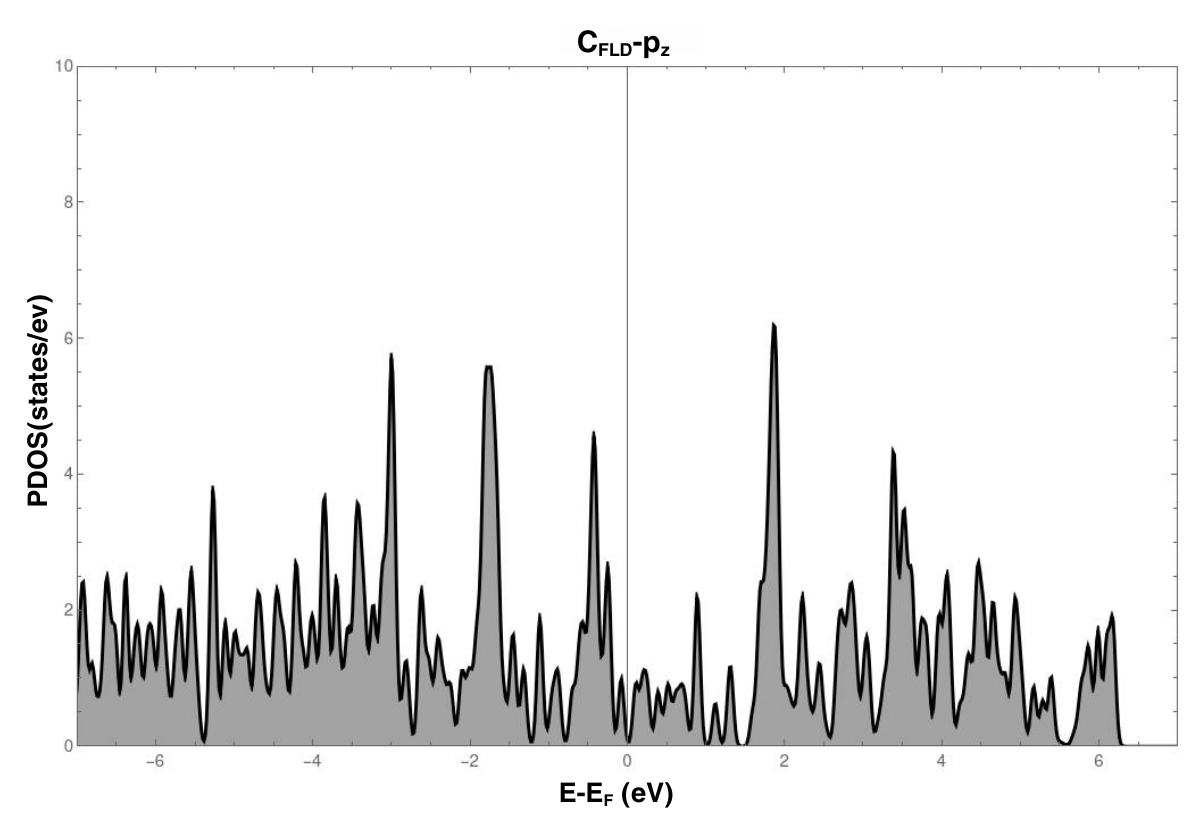
\includegraphics[scale=0.13]{../figures/CFLD-pz.png}
  \end{minipage}
  \caption{Left: Band structure of $7\times7$ FLD superlattice. Right: (Top) Density of states (DOS), (Middle) Contributtion of FLD carbon atoms to the density of states and (Bottom) Main contribution from $p_z$ orbitals around Fermi level from the FLD carbon atoms.}
  \label{fig:7x7_band}
\end{figure}

\begin{figure}[H]
  \centering
  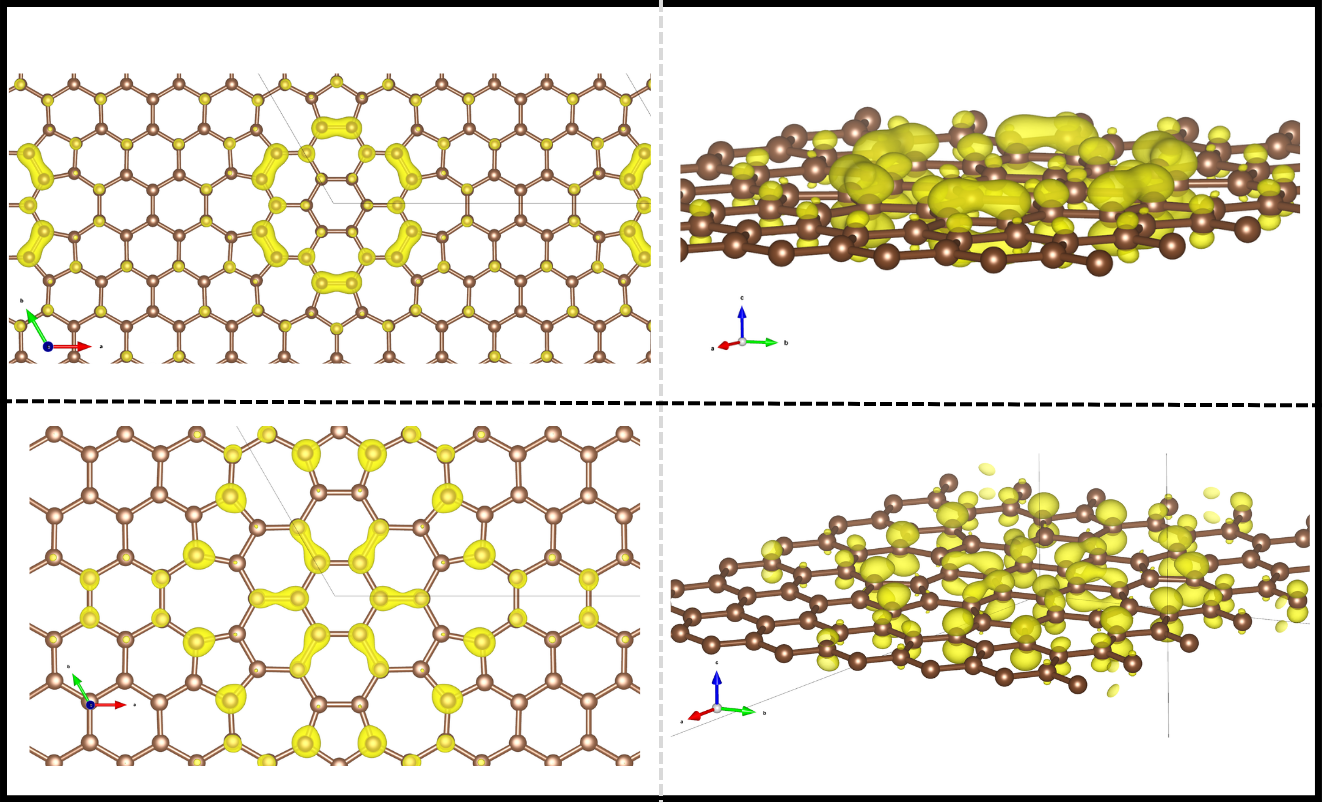
\includegraphics[scale=0.4]{../figures/parchg_7x7.png}
  \caption{Top: Isosurface images of partial charge density of last occupied band. Bottom: Isosurface images of partial charge density of first unoccupied band.}
  \label{fig:7iso}
\end{figure}

\begin{figure}[H]
  \centering
  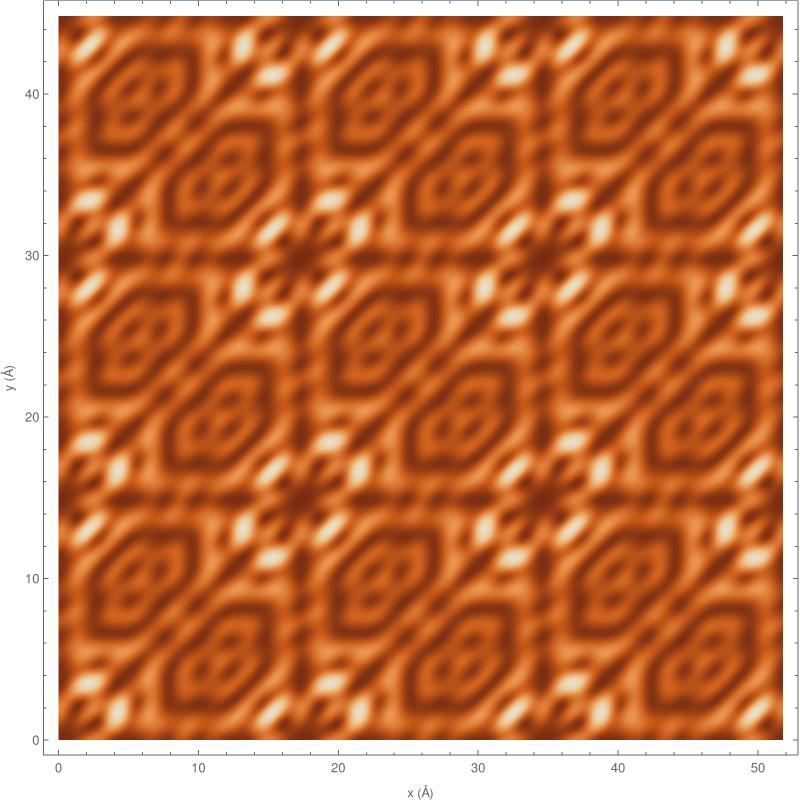
\includegraphics[scale=0.2]{../figures/stm_0.3.jpeg}
  \caption{Simulated STM image of the $7\times7$ FLD superlattice at a bias voltage of $V_{\text{bias}} = -0.3~\text{eV}$.}
  \label{fig:stm}
\end{figure}

\section{Conclusion and Future Work}
In this study, we have provided insights into the electronic properties of a 7x7 graphene superlattice with topological defects. Future work will explore vacancies in the arrangement, incorporate transition metal adatoms at different non-equivalent sites, and investigate the effects of adding a new layer in various non-equivalent configurations. These explorations will further enhance our understanding of defect-engineered graphene for potential applications in electronics and quantum technologies.


\bibliography{references}


\end{document}
